\section{Implementation}
\label{sec:implementation}

Web application development framework \textit{Django}~\cite{django} and Web API toolkit \textit{Django REST Framework} (DRF)~\cite{drf} and Python~\cite{python} library \textit{django-filter}~\cite{django-filter} were used to develop our annotation tool.
PostgreSQL~\cite{psql} is used to provide a database for the server-side applications of the software.
This database is responsible for serving the entire data needed to operate the tool, the search API, etc.
During the implementation phase, decisions regarding models of the database have been directed towards making the tool's UI make use of the APIs for database queries and searches.
The models reflect the UD format of a sentence and sentences are saved as word lines at the core.

Annotation page has all the functionalities of \boatvone\ and more.
Errors are displayed for annotators to see invalid edits in real time.
They are checked and annotations validated according to the UD framework and the language provided.
The scripts used for validation are the ones already provided by the framework as of 2022~\cite{UD-git}.

A Python library \textit{spaCy}~\cite{spacy} is used to provide linear dependency graphs.
Another JavaScript-based linear dependency graph~\cite{spyssalo} making use of \textit{brat}~\cite{brat-vis} is used to provide graphs as well.
The preferences of annotators may vary and giving them options in different parts of the screen is important.

\begin{figure}[tbh]
    \centering
    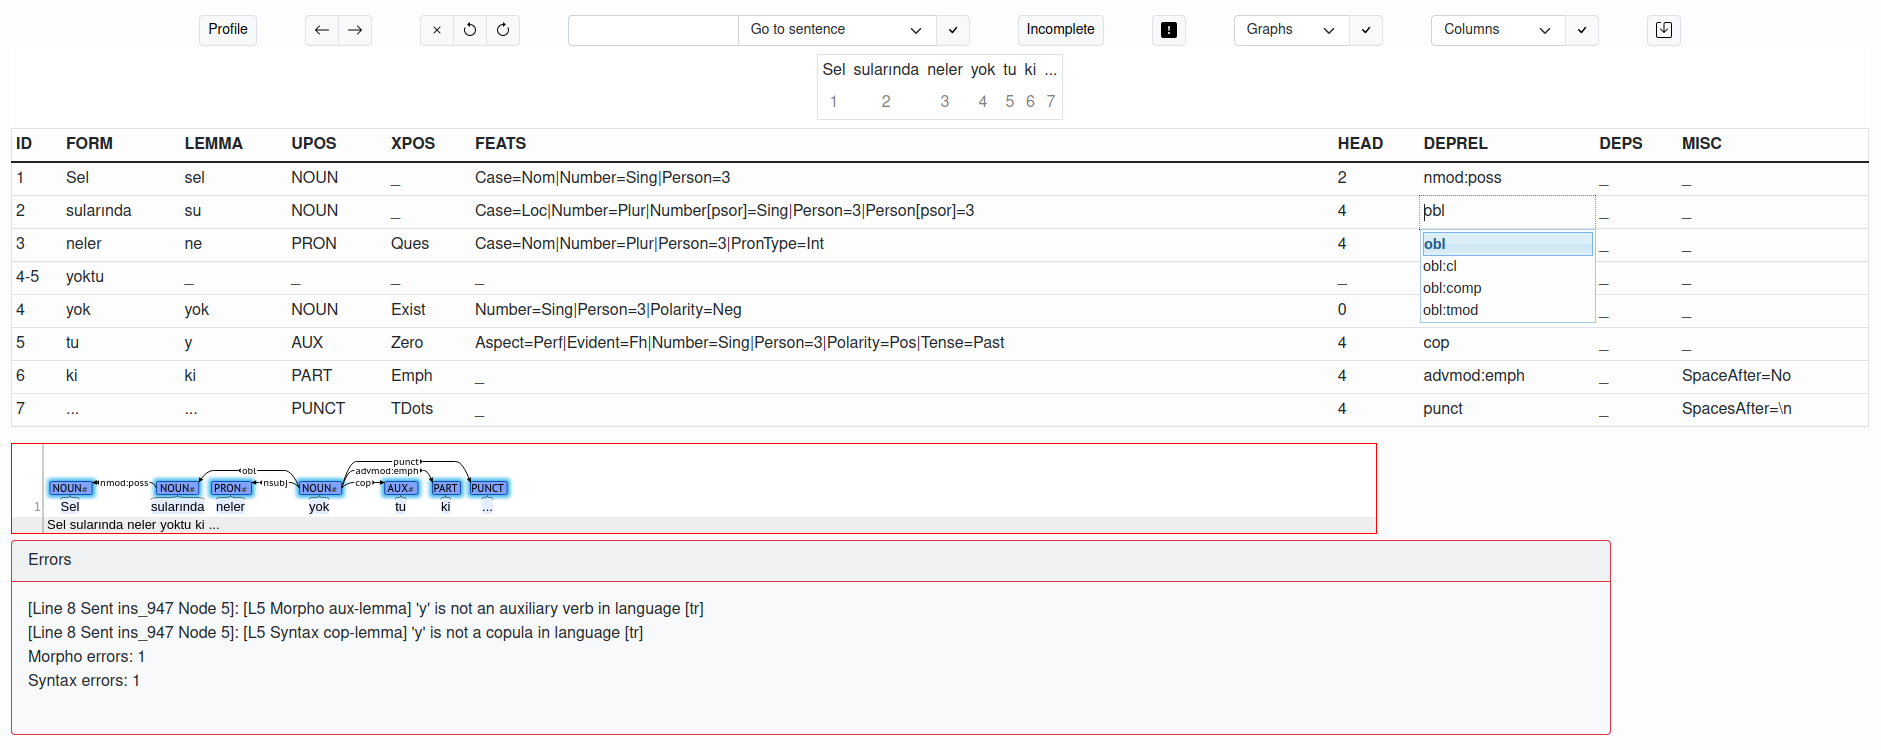
\includegraphics[width=1\textwidth]{figures/1.png}
    \caption{Annotation view for the sentence "Sel sularında neler yoktu ki..."}
    \label{fig:demo-fig}
\end{figure}

\subsection{Features}
\label{sec:features}

There are many new features and improvements in this tool, as well as the functionality that already existed in \boatvone.

\begin{itemize}[before=\normalfont, font=\itshape, align=left]
\item[Loading files:] Instead of loading a specific file before annotating, a user is able to upload a \conllu{} file to the database and start annotating.
The file is parsed and checked for its format. It's rejected if incorrectly formatted, otherwise uploaded to the database.
This way, other annotators working with the same treebank don't have to provide the same file.

\item[Annotation view:] The annotation page is very similar to \boatvone.
There is an annotation table for editing the word lines of \conllu\ files.
It includes a dependency graph and an editable table, both of which are in sync.
The dependency graph of the initial tool and other 2 graphs have been added to this tool.
The user has the choice to select a type of graph or none.
The other 2 graphs, which are both horizontal and linear, have been selected due to space considerations.

\item[Network-enabled Search:] An important feature in this version is the ability to cross-check annotations by implementing a network for annotators where they can review the annotations done by other annotators and if they disagree on some parts, they can interact outside the tool.
This can be helpful and a learning experience for annotators.

For an actual example, the annotator, responsible for the \bountreebank{}'s annotation, was annotating a sentence that had a Zodiac sign noun.
Not being sure about how to annotate the noun's \textit{UPOS} tag, she searched for similar cases in the \conllu{} file and encountered two different ways nouns of Zodiac signs were annotated previously.
Besides not helping how to choose a \textit{UPOS} tag, this raises a consistency issue within the treebank as well.
One of the nouns was annotated as \textit{NOUN} in its \textit{UPOS} tag, the other one was as \textit{PROPN}.
The annotator searched the \conllu{} file in a text editor and decided to use the one with the more cases of annotation and proceeded to replace the inconsistent ones with the current decision.
This case can be handled by a simple search of the database.
We provide a search page and API in this tool where treebanks can be searched by \textit{sent\_id}s, \textit{text}s, all the UD tags and treebank names.
With this, an annotator can easily make the treebank more consistent and reduce their frustration.

Another example could be given by the various -ki morphemes in Turkish.
In the sentence "Evdeki halılar yıkandı." (\textit{"The rugs at home were washed."}), the -ki acts as an adjectivizer.
In another sentence "Benim halılarım yün, Ayşeninkiler sentetik." (\textit{"My rugs are wool. Ayse's are synthetic."}), it is pronominal.
An annotator might not recall how a specific -ki morpheme should be annotated and a single search would be a big help.

Also one other thing the inter-annotator agreement allows us is the possibility to see some anomalies in the Turkish part of the validation of the UD framework.
For example, if a sentence were annotated a way by many annotators but the UD validation script were finding it invalid, this might indicate the UD validation were lacking in this respect of the Turkish language.
Some modifications might be necessary and there could be a case for a proposal of change.

\item[Annotation status:] We also provide a feature where an annotation has a status regarding it completeness.
There are 3 different statuses and they are cycled through by the annotator in the annotation view.
Status of an annotation is also shown in the search view, helping to select an appropriate case.
Also there is another view where an annotator can list their completed, drafted or incomplete annotations, helping to keep track of what annotations have already been completed.

\end{itemize}
